\chapter{Protocolos y variantes de referencia}\label{app:procedencia}

\section{Separación de evaluaciones}
Las 47 condiciones estáticas por clasificador incluyen tres semillas en FMD y Soil. El panel canónico de 27 conserva solo la semilla 42 en esos conjuntos. Las medias de ambos paneles pueden diferir sin que una tabla reemplace a la otra. El piloto híbrido produce predicciones OOF de las 680 imágenes del entrenamiento oficial de Outex y mantiene fuera su test oficial.

En los experimentos de desarrollo anteriores de DTD se utilizó también una partición SGKF de 4.512/1.128 imágenes. Su entrenamiento incluye 1.501 imágenes del test oficial 1, por lo que esas exploraciones no se presentan como evaluación oficial ciega ni como controles directos del benchmark. No se mezclan sus métricas con las tablas principales.

\section{Procedencia de KTH}
Las tablas estáticas conservan los resultados archivados de 22 bloques. El Top-$k$ SVM de origen registra macro-F1 medio aproximado de 0,9400; el control corregido con agrupación interna por muestra registra aproximadamente 0,9445. La cascada se construyó con el rescate anterior. Coincidir en una media no acredita que selecciones, transformaciones y predicciones sean idénticas.

Los contrastes estáticos sobre seis conjuntos describen el archivo indicado; no certifican que todos sus controles correspondan a la variante KTH corregida. La inferencia conjunta de la cascada excluye KTH hasta reconciliar su ruta completa. Tampoco se sustituye solo una cifra en el análisis para resolver esta reserva.

\section{Fidelidad de los pilotos físicos}
El piloto de una condición por conjunto se documenta con registros por imagen y repetición. La coincidencia de rutas o clases no basta para establecer identidad del vector extraído. CUReT y Soil mantienen cosenos mínimos aproximados de -0,0707 y 0,0085 respecto al caché. No se atribuye la diferencia a una capa, interpolación o normalización concreta sin diagnóstico controlado.

\section{Particiones y multiplicidades del piloto híbrido}
El desarrollo utiliza únicamente las 680 imágenes del entrenamiento oficial de Outex. Los pliegues productores estratificados y agrupados usan semilla 142; los internos, semilla 42. Cada ensamble contiene 15 votos, pero un subconjunto repetido reutiliza el mismo modelo y conserva su multiplicidad en la agregación.

\begin{table}[!htbp]
\centering\small
\caption{Tamaños y modelos únicos del control de diversidad permanente en cada pliegue productor. No son nuevas réplicas ni 15 ejecuciones distintas por imagen.}
\label{tab:producer-folds}
\begin{tabular}{@{}lrrrr@{}}
\toprule
Pliegue & Entrenamiento & Validación & Votos & Modelos únicos\\
\midrule
0 & 453 & 227 & 15 & 9\\
1 & 453 & 227 & 15 & 11\\
2 & 454 & 226 & 15 & 12\\
\bottomrule
\end{tabular}
\end{table}

El sorteo de diversidad usa las semillas 4.200.009, 4.200.019 y 4.200.029, derivadas de la semilla de desarrollo y del índice productor. Las particiones y miembros se conservan en los registros por pliegue. Un modelo único del rescate no equivale a un extractor único: su costo depende de la unión de los cuatro bloques de cada miembro, descontando la base cuando ya está adquirida.

\section{Figuras de la cascada de referencia}
\begin{figure}[!htbp]
\centering
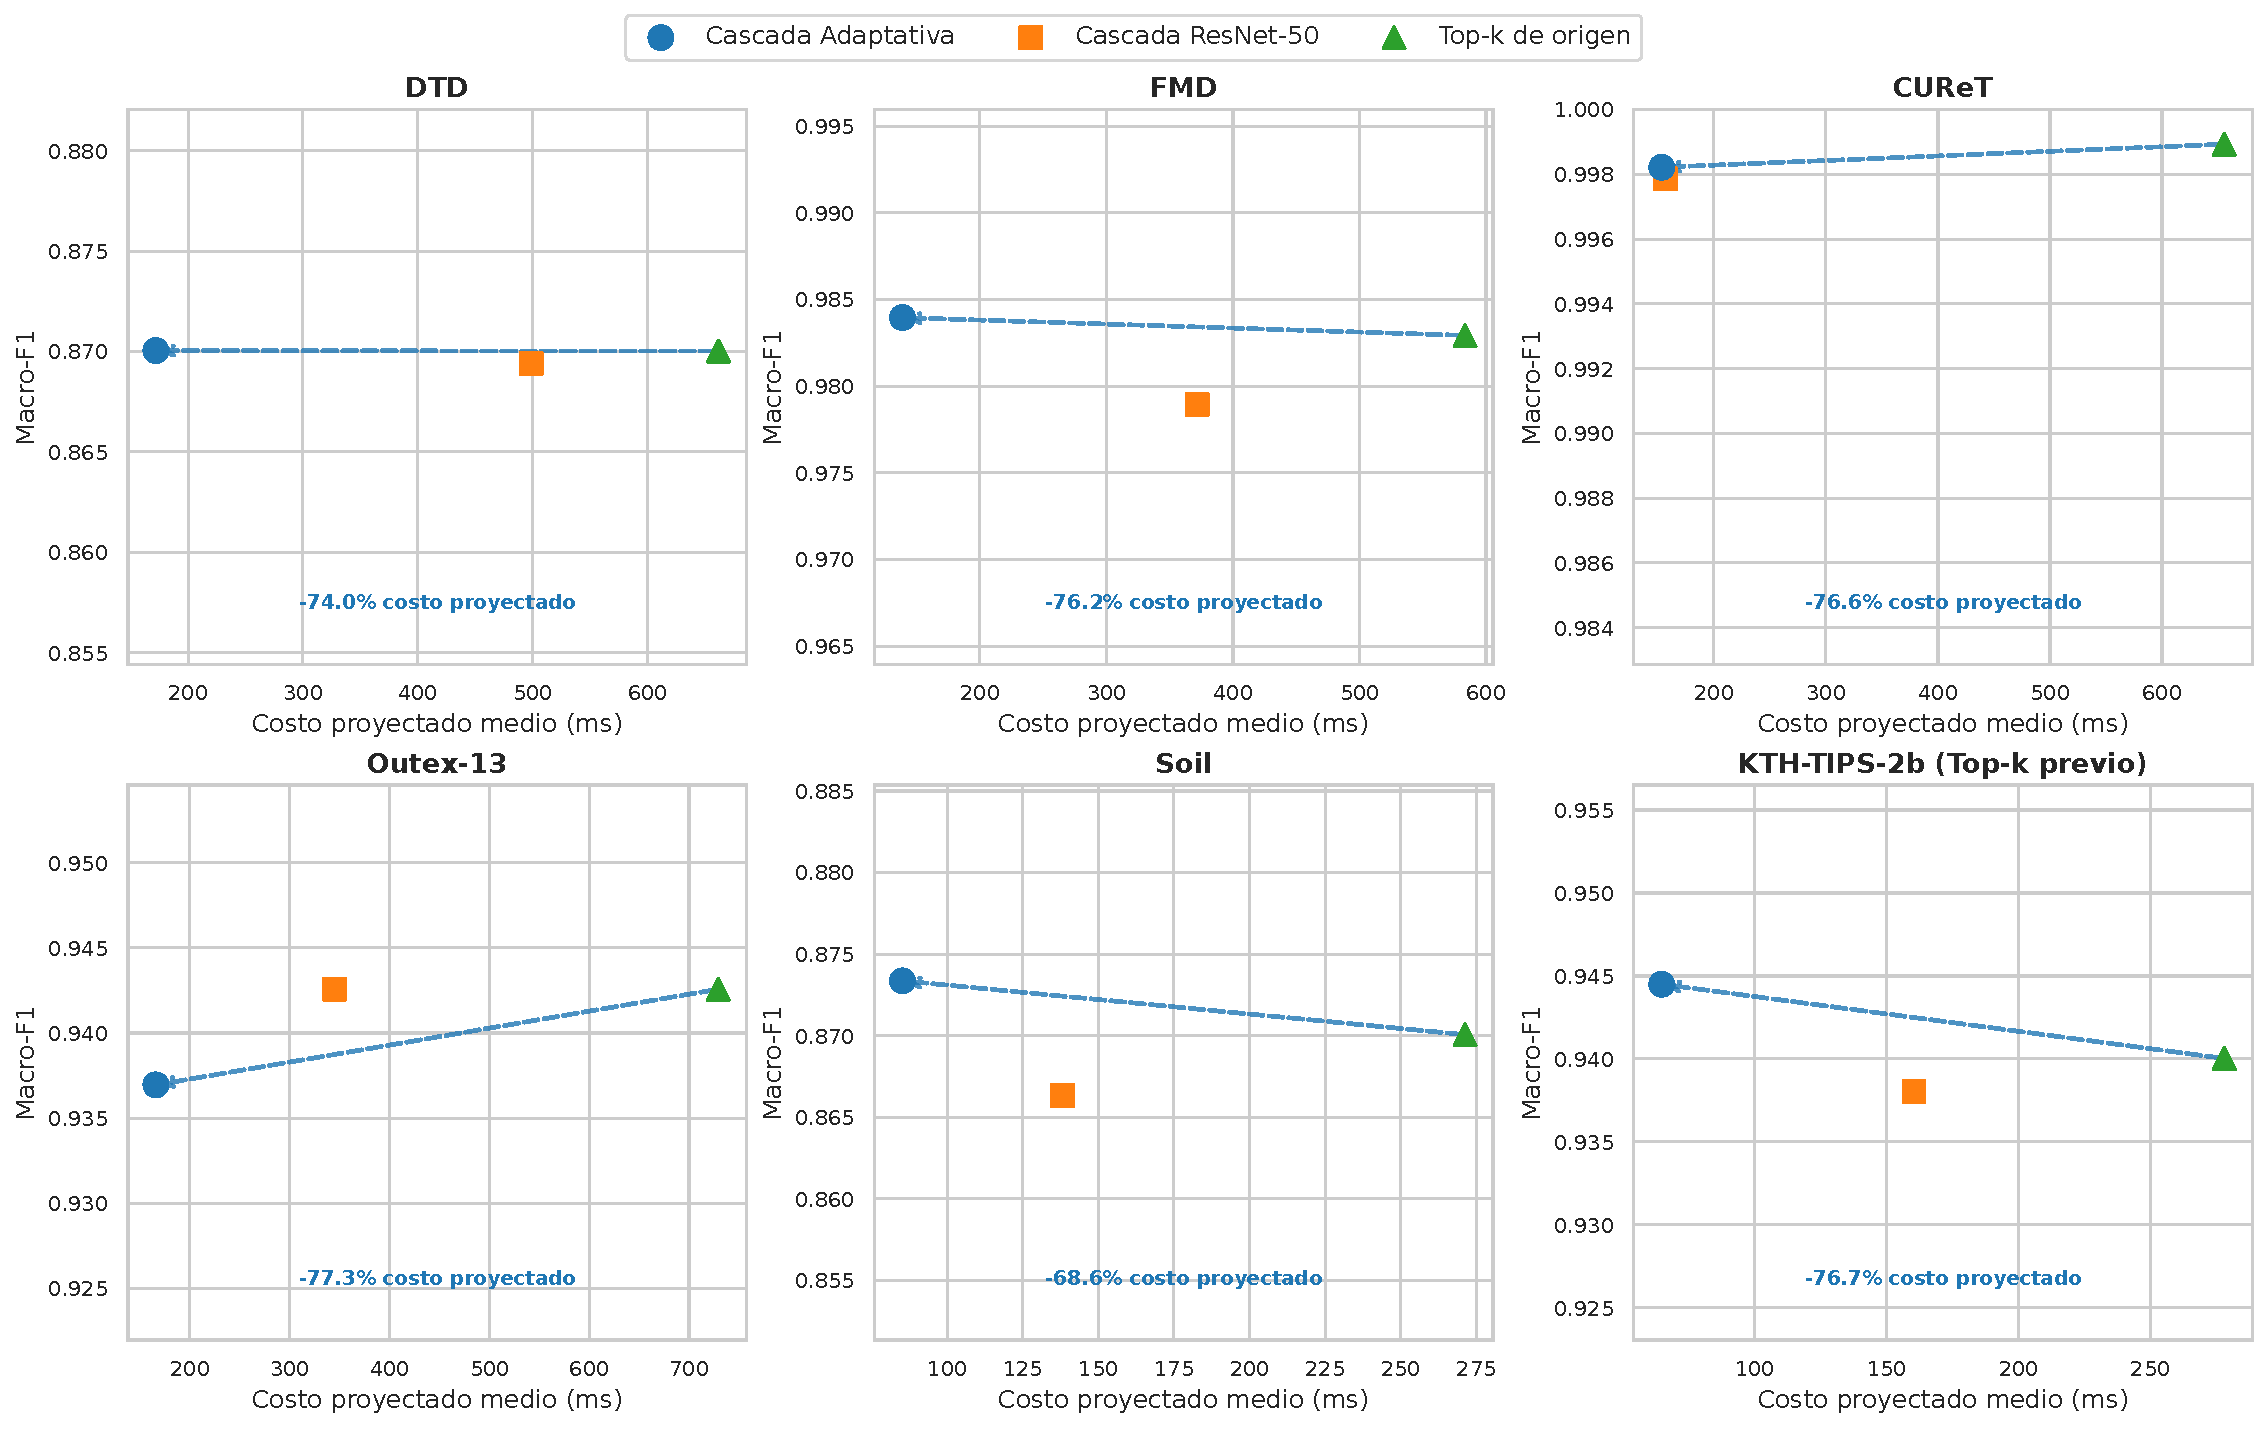
\includegraphics[width=0.85\textwidth]{figures/pareto_frontier_adaptive_cascade.pdf}
\caption{Comparación histórica calidad--costo bajo su perfil analítico. No representa el rescate de diversidad ni una medición física de todas las rutas.}
\label{fig:pareto-cascade}
\end{figure}
\begin{figure}[!htbp]
\centering
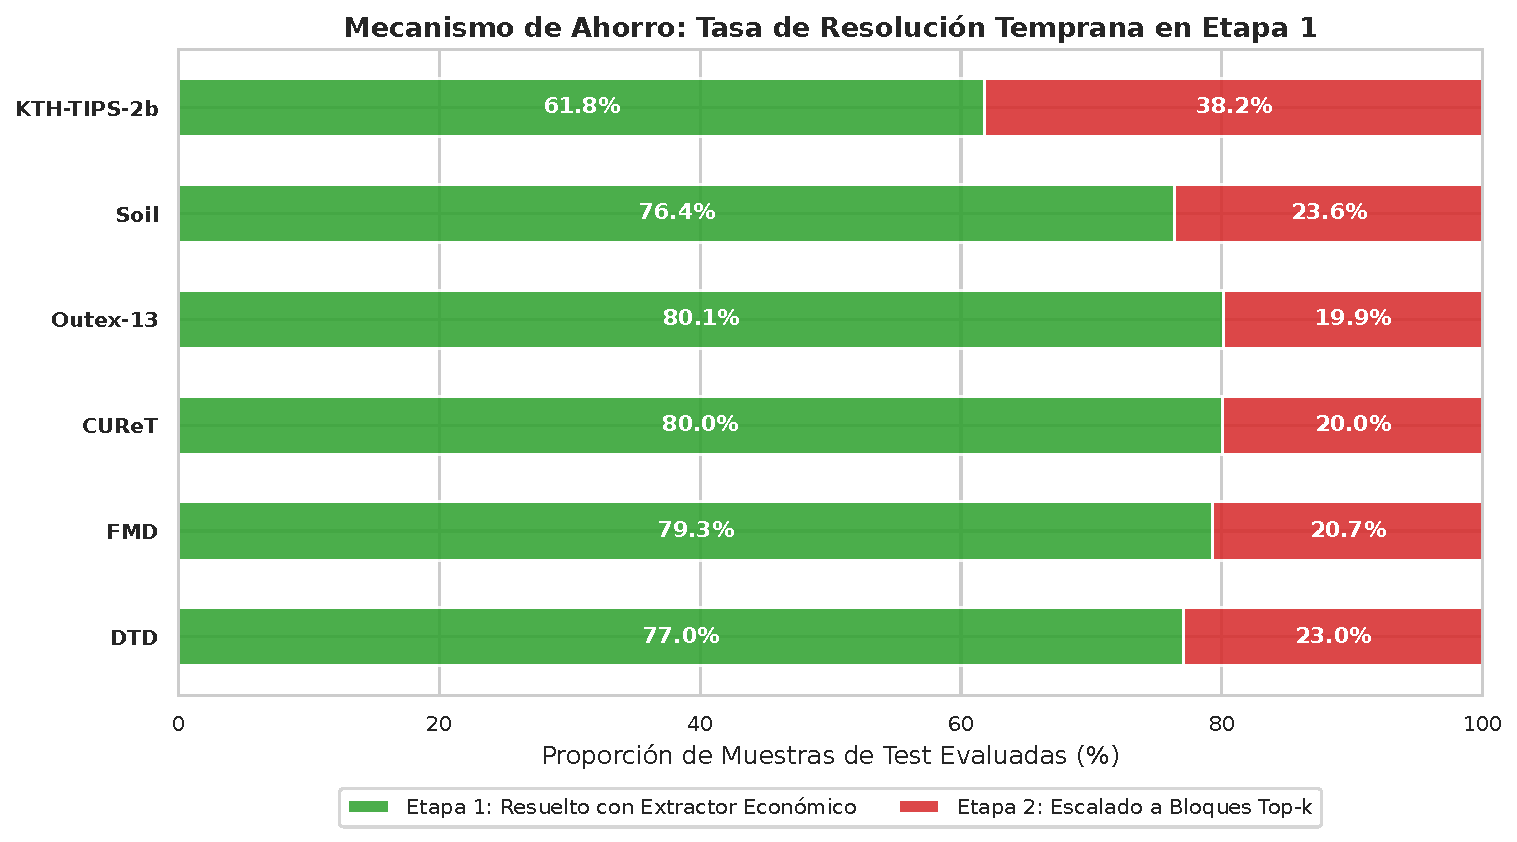
\includegraphics[width=0.85\textwidth]{figures/cascade_routing_efficiency.pdf}
\caption{Enrutamiento de la cascada histórica según los artefactos archivados. Las proporciones no garantizan una tasa de salida para imágenes nuevas.}
\label{fig:routing-efficiency}
\end{figure}


\FloatBarrier
